\documentclass[11pt,a4paper]{article}
\usepackage[utf8]{inputenc}
\usepackage[T1]{fontenc}
\usepackage{geometry}
\usepackage{graphicx}
\usepackage{hyperref}
\usepackage{booktabs}
\usepackage{parskip}
\usepackage{tikz}
\usepackage{seqsplit}
\usepackage{listings}
\usepackage{xcolor}
\usepackage{float}
\usepackage{tabularx}
\usepackage{makecell}
\usetikzlibrary{shapes.geometric, arrows.meta, positioning}
\geometry{margin=2.5cm}
\sloppy

% Python listings configuration
\lstset{
  language=Python,
  basicstyle=\ttfamily\small,
  keywordstyle=\color{blue},
  commentstyle=\color{gray}\itshape,
  stringstyle=\color{red},
  showstringspaces=false,
  breaklines=true,
  frame=single,
  numbers=left,
  numberstyle=\tiny,
  xleftmargin=2em,
  framexleftmargin=1.5em,
  literate={\#}{{\#}}1,
}

\title{Web Data Mining and Semantics\\Report: Final Project}
\author{Gabriel SULTAN - A4 - DIA 6}
\date{March 2026}

\begin{document}
\maketitle

%=============================================================================
\section{Introduction}
%=============================================================================

This report describes a complete pipeline for building a Knowledge Base (KB) in the domain of \textbf{Local History} (monuments, historical figures, places), from raw web data to a structured RDF graph aligned with Linked Open Data (LOD). The pipeline integrates four lab sessions: Data Acquisition \& Information Extraction (Phase~1), KB Construction \& Expansion (Phase~2), Knowledge Reasoning with SWRL and KGE (Phase~3), and RAG over RDF/SPARQL (Phase~4).

\textbf{Data source.} We use the \textbf{Europeana API} (and Wikidata) as the primary source. Europeana provides metadata for millions of digitized cultural heritage items; extracting text from the Search API JSON response avoids anti-robot issues and simplifies content extraction compared to HTML scraping.

\textbf{Running the full pipeline.} From the project root: \texttt{python run\_pipeline.py} runs Phases~1--2 (crawler $\rightarrow$ IE $\rightarrow$ build KB $\rightarrow$ entity linking $\rightarrow$ predicate alignment $\rightarrow$ expansion). Phase~3: open \texttt{src/kge/phase3\_knowledge\_reasoning.ipynb}. Phase~4: \texttt{python src/rag/lab\_rag\_sparql\_gen.py} (Ollama required).

%=============================================================================
\section{Data Acquisition \& Information Extraction}
%=============================================================================

\subsection{Domain and Seed URLs}

Domain: \textbf{Local History} (cultural heritage objects). Per Phase~1 instructions (5--10 seed URLs), we use the Europeana Search API with queries as equivalent ``seeds'': \texttt{Paris history}, \texttt{Notre-Dame Paris}, \texttt{Eiffel Tower}, \texttt{Louvre Museum}, \texttt{Palace of Versailles}, \texttt{Arc de Triomphe Paris}, \texttt{Bastille Paris}, \texttt{Sainte-Chapelle Paris}. Each query returns multiple records, items with $\geq$500 words are kept.

\textbf{Execution.} From the project root: \texttt{python src/crawl/phase1\_crawler.py}. Queries are defined in \texttt{config.py}:

\begin{lstlisting}[caption={\texttt{config.py} (excerpt) -- seeds and User-Agent}]
EUROPEANA_QUERIES = [
    "Paris history", "Notre-Dame Paris", "Eiffel Tower",
    "Louvre Museum", "Palace of Versailles", ...
]
USER_AGENT = "WebMiningSemanticsStudent/1.0 (Educational project; Python/httpx)"
MIN_WORD_COUNT_API = 500
\end{lstlisting}

\subsection{Crawler Design and Ethics}

Per instructions, we use APIs when anti-robot checking occurs. The crawler respects web ethics:
\begin{itemize}
\item identifiable \texttt{User-Agent} (\texttt{WebMiningSemanticsStudent/1.0})
\item robots.txt check via \texttt{urllib.robotparser} before fetching
\item rate limiting to avoid overloading the API
\end{itemize}
No trafilatura is needed because text is extracted directly from the JSON response. The corresponding code is in \texttt{src/crawl/phase1\_crawler.py}:

\begin{lstlisting}[caption={\texttt{src/crawl/phase1\_crawler.py} -- robots.txt and User-Agent}]
def _is_allowed_by_robots(url, user_agent, robots_cache):
    parsed = urlparse(url)
    domain = f"{parsed.scheme}://{parsed.netloc}"
    rp = robotparser.RobotFileParser()
    resp = client.get(robots_url, headers={"User-Agent": user_agent})
    rp.parse(resp.text.splitlines())
    return rp.can_fetch(user_agent, url)
# Call: headers={"User-Agent": config.USER_AGENT}
\end{lstlisting}

\subsection{Cleaning Pipeline}

The extraction pipeline: First, flatten text from nested API payloads; Second, filter URL literals (not useful for NLP); Then, normalize whitespace; Finally, apply a useful-page threshold ($\geq$500 words). Results are stored in JSONL format (\texttt{url}, \texttt{text}, \texttt{title}, \texttt{word\_count}). Implementation in \texttt{src/crawl/phase1\_crawler.py}:

\begin{lstlisting}[caption={\texttt{src/crawl/phase1\_crawler.py} -- cleaning: flatten, filter URLs, 500-word threshold}]
def _build_text_from_item(item):
    values = _flatten_text_values(item)
    cleaned = []
    for v in values:
        s = str(v).strip()
        if _is_http_url(s): continue  # URLs not useful for NLP
        cleaned.append(s)
    text = re.sub(r"\s+", " ", " ".join(cleaned)).strip()
    return text
# Filter: word_count < config.MIN_WORD_COUNT_API (500) -> skip
\end{lstlisting}

\subsection{NER and Relation Extraction}

\textbf{NER.} We use spaCy with \texttt{en\_core\_web\_trf} (transformer-based) to extract PERSON, ORG, GPE, and DATE. Common nouns are filtered out. The lemmatizer normalizes verb forms for consistent predicate naming.

\textbf{Relations.} For each sentence with at least two entities, we use dependency tags (\texttt{nsubj}, \texttt{dobj}, \texttt{pobj}) to find a verb connecting them. Example: ``Marie Curie discovered Polonium'' $\rightarrow$ \texttt{(Marie Curie, discovered, Polonium)}. When no verb is found, we use \texttt{relatedTo} as fallback.

\textbf{Execution:} \texttt{python src/ie/phase1\_extraction.py}. File: \texttt{src/ie/phase1\_extraction.py}.

\begin{lstlisting}[caption={\texttt{src/ie/phase1\_extraction.py} -- NER and relation extraction (dependencies)}]
ENTITY_LABELS = {"PERSON", "ORG", "GPE", "DATE"}
for ent in doc.ents:
    if ent.label_ not in ENTITY_LABELS: continue
    # FILTER_ENTITIES, _is_valid_entity to avoid false positives
for sent in doc.sents:
    for token in sent:
        subjs = [c for c in token.children if c.dep_ in ("nsubj","nsubjpass")]
        objs = [c for c in token.children if c.dep_ in ("dobj","pobj","attr")]
        if (s in e1 and o in e2): verb = token.lemma_
\end{lstlisting}

\begin{figure}[H]
\centering
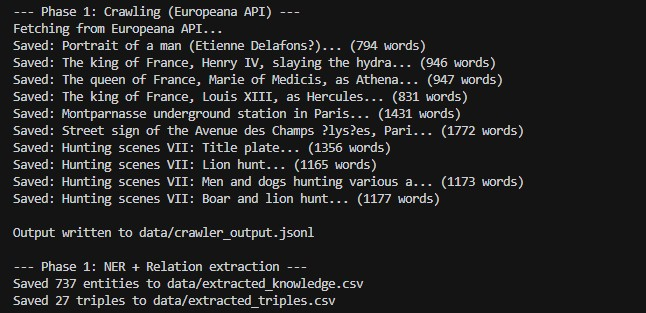
\includegraphics[width=0.95\textwidth]{../screenshots/phase1.jpg}
\caption{Phase 1 pipeline output: Europeana API crawling (10 records saved to \texttt{data/crawler\_output.jsonl}) and NER + relation extraction (797 entities to \texttt{extracted\_knowledge.csv}, 18 triples to \texttt{extracted\_triples.csv}).}
\end{figure}

\begin{figure}[ht]
\centering
\resizebox{\linewidth}{!}{%
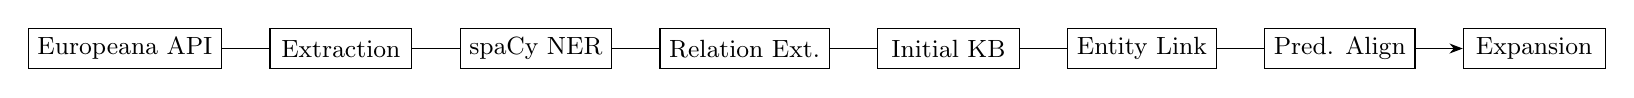
\begin{tikzpicture}[
  node distance=0.6cm,
  box/.style={rectangle, draw, minimum width=1.8cm, minimum height=0.5cm, font=\small},
  arrow/.style={-Stealth}
]
  \node[box] (api) {Europeana API};
  \node[box, right=of api] (extract) {Extraction};
  \node[box, right=of extract] (ner) {spaCy NER};
  \node[box, right=of ner] (re) {Relation Ext.};
  \node[box, right=of re] (kb) {Initial KB};
  \node[box, right=of kb] (el) {Entity Link};
  \node[box, right=of el] (pa) {Pred. Align};
  \node[box, right=of pa] (exp) {Expansion};
  \draw[arrow] (api) -- (extract) -- (ner) -- (re) -- (kb) -- (el) -- (pa) -- (exp);
\end{tikzpicture}%
}
\caption{Global pipeline: Phase~1 (Crawling $\rightarrow$ NER $\rightarrow$ RE) and Phase~2 (KB $\rightarrow$ alignment $\rightarrow$ expansion).}
\end{figure}

\subsection{Entity Ambiguity: Three Examples}

\begin{enumerate}
\item \textbf{``Paris''} --- Can denote the city (GPE), a person (Paris Hilton), or a document (Treaty of Paris). Context is crucial; the model may mislabel in ambiguous sentences.

\item \textbf{``May''} --- May be a month (DATE), a person's name (PERSON), or a modal verb. In ``The treaty was signed in May 1919,'' it is correctly a DATE. In ``May I help you?,'' it is not an entity.

\item \textbf{``Louis''} --- In ``Louis XIV built the Palace of Versailles,'' Louis refers to the king. In ``Louis, Missouri,'' it refers to a place. The model may confuse ``Louis'' with ``Saint Louis'' (person or city). Without disambiguation, entity linking can fail.
\end{enumerate}

We apply type-based filtering (GPE $\rightarrow$ place, PERSON $\rightarrow$ human) and Property Evidence when available to improve disambiguation during entity linking.

\subsection{Scaling Reflection}

For 10,000 pages instead of 10: (1)~parallel crawling with \texttt{asyncio} and rate limiting; (2)~incremental JSONL storage and batch NER; (3)~database (SQLite) for entity/triple storage; (4)~resumability (track crawled URLs, checkpoints); (5)~monitoring with exponential backoff.

%=============================================================================
\section{KB Construction \& Alignment}
%=============================================================================

\subsection{RDF Modeling Choices}

The initial KB uses URIs (not plain strings), camelCase predicates (\texttt{relatedTo}), and separates entities from literals. New entities receive ontological definitions (Person, Place, Organization, Temporal) in \texttt{ontology.ttl}.

\textbf{Execution:} \texttt{python src/kg/phase2\_build\_kb.py}. File: \texttt{src/kg/phase2\_build\_kb.py}.

\begin{lstlisting}[caption={\texttt{src/kg/phase2\_build\_kb.py} -- initial KB construction (URIs, camelCase)}]
NS = Namespace("http://example.org/localhistory/")
type_map = {"PERSON":"Person","ORG":"Organization","GPE":"Place","DATE":"Temporal"}
for _, row in entities_df.iterrows():
    subj = URIRef(NS[to_uri(row["entity"])])
    g.add((subj, RDF.type, NS[type_map.get(row["entity_type"],"Thing")]))
for _, row in triples_df.iterrows():
    g.add((URIRef(NS[s]), NS[to_predicate(row["predicate"])], URIRef(NS[o])))
\end{lstlisting}

\subsection{Entity Linking with Confidence}

We search the Wikidata API (\texttt{wbsearchentities}). When a match is found, we add \texttt{owl:sameAs} to the Wikidata URI with the confidence returned by the API. The mapping table (\texttt{mapping\_table.csv}) records private entity $\rightarrow$ Wikidata URI with confidence. Entities not found in Wikidata are created in the ontology and marked as NEW. Disambiguation: type-based filtering, Property Evidence, and label match.

\textbf{Execution:} \texttt{python src/kg/phase2\_entity\_linking.py}. File: \texttt{src/kg/phase2\_entity\_linking.py}.

\begin{lstlisting}[caption={\texttt{src/kg/phase2\_entity\_linking.py} -- entity linking with confidence (Wikidata API)}]
def search_wikidata_entity(label, entity_type=None):
    params = {"action":"wbsearchentities","search":label,"limit":5}
    if wlabel.lower() == label.strip().lower(): conf = 0.95
    elif match_type == "label": conf = 0.92
    else: conf = 0.85 - (i * 0.05)
    if hints and any(h in desc for h in hints): conf = min(0.98, conf + 0.05)
    results.append((uri, conf))
# alignment.add((URIRef(NS[lh_name]), OWL.sameAs, URIRef(uri)))
\end{lstlisting}

\subsection{Predicate Alignment}

We use SPARQL on \texttt{query.wikidata.org} to find equivalent properties. For each private predicate, we query by label (e.g.\ ``location'' for \texttt{locatedIn}) and select the most pertinent result. We use \texttt{owl:equivalentProperty} when semantics match exactly, and \texttt{rdfs:subPropertyOf} when our predicate is narrower. Manual priority mapping for key predicates: \texttt{locatedIn} $\rightarrow$ \texttt{wdt:P276}, \texttt{build/design} $\rightarrow$ \texttt{wdt:P170}, \texttt{crown} $\rightarrow$ \texttt{wdt:P166}. Fallback: EDM/Dublin Core (\texttt{dcterms:spatial}, \texttt{dc:creator}).

\textbf{Execution:} \texttt{python src/kg/phase2\_predicate\_alignment.py}. File: \texttt{src/kg/phase2\_predicate\_alignment.py}.

\begin{lstlisting}[caption={\texttt{src/kg/phase2\_predicate\_alignment.py} -- predicate alignment (SPARQL Wikidata + EDM)}]
PREDICATE_TO_WIKIDATA = {
    "locatedIn": WDT["P276"], "build": WDT["P170"], "crown": WDT["P166"], ...
}
def sparql_wikidata_property(search_term, limit=10):
    query = "SELECT ?property ?propertyLabel WHERE {...}"
    resp = client.get(WIKIDATA_SPARQL, params={"query":query})
if wd_uri: alignment.add((lh_pred, OWL.equivalentProperty, wd_uri))
else: alignment.add((lh_pred, OWL.equivalentProperty, edm_uri))
\end{lstlisting}

\begin{figure}[H]
\centering
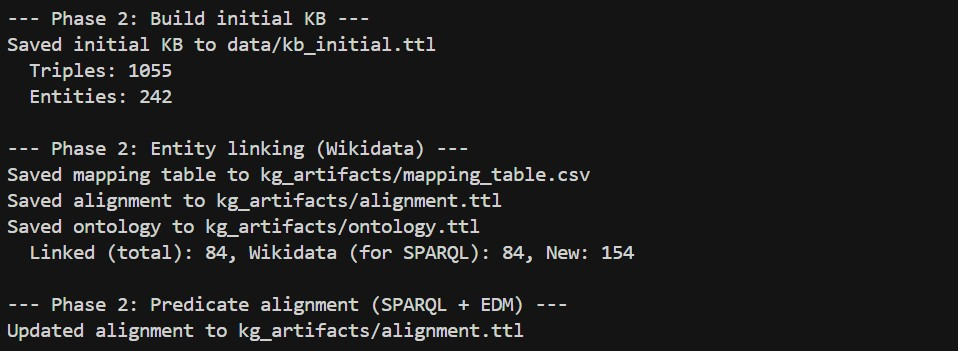
\includegraphics[width=0.95\textwidth]{../screenshots/phase2_to_pred.jpg}
\caption{Phase 2 pipeline output (build KB, entity linking, predicate alignment): initial KB (1,055 triples, 242 entities), entity linking (84 linked to Wikidata, 154 new), alignment updated to \texttt{kg\_artifacts/alignment.ttl}.}
\end{figure}

\subsection{Expansion Strategy}

Entity linking $\rightarrow$ subgraph extraction via SPARQL $\rightarrow$ merge. (1)~\textbf{1-Hop:} For aligned entities (confidence $\geq$ 0.85), \texttt{SELECT ?p ?o WHERE \{ wd:Qxxx ?p ?o \} LIMIT 1000} with a predicate whitelist. (2)~\textbf{2-Hop:} Sample of entities, triples via intermediate nodes. (3)~\textbf{Predicate-controlled:} \texttt{SELECT ?s ?p ?o WHERE \{ ?s wdt:Pxxx ?o \}} for key properties. (4)~\textbf{Europeana complement:} If volume $<$ 50k triplets, add Europeana API records. (5)~\textbf{Cleanup:} Fix malformed literals, deduplicate, export to N-Triples.

\textbf{Execution:} \texttt{python src/kg/phase2\_expand\_kb.py} (or \texttt{--quick} for test). Files: \texttt{src/kg/phase2\_expand\_sparql.py}, \texttt{src/kg/phase2\_expand\_kb.py}.

\begin{lstlisting}[caption={\texttt{src/kg/phase2\_expand\_sparql.py} -- SPARQL 1-Hop and 2-Hop}]
def sparql_1hop(qid, limit=1000):
    query = "SELECT ?p ?o WHERE { wd:"+qid+" ?p ?o } LIMIT "+str(limit)
def sparql_2hop(qid, limit=500):
    query = "wd:"+qid+" ?p1 ?intermediate . ?intermediate ?p ?o"
# qids = get_wikidata_qids_from_mapping(mapping_path, min_confidence=0.85)
\end{lstlisting}

\begin{figure}[H]
\centering
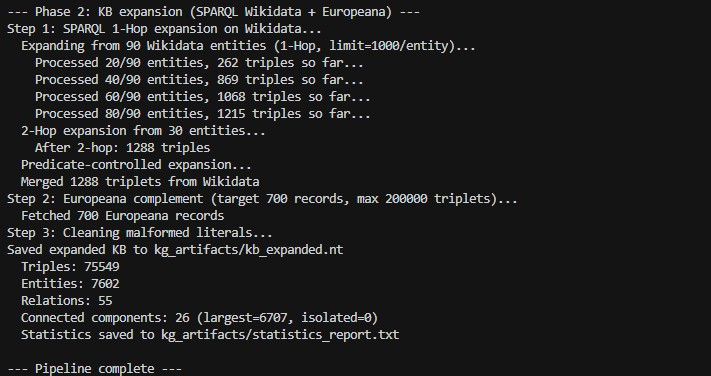
\includegraphics[width=0.95\textwidth]{../screenshots/phase2_Last_Part.jpg}
\caption{Phase 2 KB expansion output: SPARQL 1-Hop and 2-Hop on Wikidata (572 triples merged), Europeana complement (700 records), cleaning; final KB: 109,474 triples, 7,310 entities, 50 relations.}
\end{figure}

\subsection{Final KB Statistics}

From \texttt{kg\_artifacts/statistics\_report.txt}:

\begin{itemize}
\item \textbf{Triplets:} 109,474
\item \textbf{Entities:} 7,310
\item \textbf{Relations:} 50
\item \textbf{Connected components:} 16; largest component: 6,904; isolated entities: 0
\end{itemize}

These values satisfy the target (50k--200k triplets, 5k--30k entities, 50--200 relations). Europeana contributes substantially: without it, the volume would drop to $\sim$1,600 triplets. Predicate whitelisting and consolidation ensure the relation count stays within 50--200.

\subsection{Challenges and Refinements}

\textbf{Entity name normalization:} Spaces, apostrophes, special characters $\rightarrow$ URI-safe form. \textbf{Predicate semantics:} EDM properties may differ from extracted predicates; manual validation required. \textbf{Multilingual filtering:} False positives in Polish, German, Dutch mitigated via \texttt{FILTER\_ENTITIES}, \texttt{FILTER\_FRAGMENTS}, and sentence-level language heuristics. \textbf{Literal cleaning:} URL values stored as literals filtered; malformed JSON artifacts removed.

%=============================================================================
\section{Reasoning (SWRL)}
%=============================================================================

\subsection{Reasoning on family.owl (SWRL intent, OWL~DL + HermiT)}

The pedagogical target is the SWRL rule: a person older than 60 is an \texttt{oldPerson}: \texttt{Person(?p), age(?p, ?a), greaterThan(?a, 60) -> oldPerson(?p)}. \textbf{HermiT} (default in OWLReady2's \texttt{sync\_reasoner}) does not support SWRL built-ins such as \texttt{greaterThan}; \textbf{Pellet} (\texttt{sync\_reasoner\_pellet}) would, but can fail on some Java versions bundled with OWLReady2. We therefore express the \textbf{same condition in OWL~DL}: \texttt{oldPerson} $\equiv$ \texttt{Person} $\sqcap$ $\exists$\texttt{age}.(\texttt{xsd:int}, minExclusive 60), then run \texttt{sync\_reasoner()} (HermiT). \textbf{Result:} Peter (age~70) and Marie (age~69) are inferred as \texttt{oldPerson}.

\textbf{Execution:} Open and run \texttt{src/kge/phase3\_knowledge\_reasoning.ipynb}. OWL file: \texttt{kg\_artifacts/family.owl}.

\begin{lstlisting}[caption={\texttt{src/kge/phase3\_knowledge\_reasoning.ipynb} -- OWL DL equivalent SWRL (Phase 3)}]
from pathlib import Path
from owlready2 import get_ontology, sync_reasoner, ConstrainedDatatype
FAMILY_OWL_PATH = Path("../../kg_artifacts/family.owl")
onto = get_ontology(str(FAMILY_OWL_PATH.absolute())).load()
with onto:
    onto.oldPerson.equivalent_to.append(
        onto.Person & onto.age.some(ConstrainedDatatype(int, min_exclusive=60))
    )
sync_reasoner(infer_property_values=True)
for p in onto.oldPerson.instances(): print(p.name, p.age)  # Peter 70, Marie 69
\end{lstlisting}

\begin{figure}[ht]
\centering
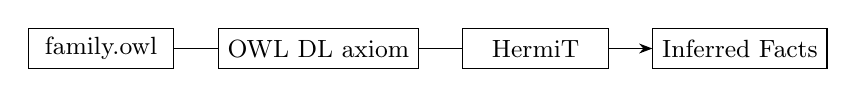
\begin{tikzpicture}[
  node distance=0.55cm,
  box/.style={rectangle, draw, minimum width=1.85cm, minimum height=0.5cm, font=\small},
  arrow/.style={-Stealth}
]
  \node[box] (owl) {family.owl};
  \node[box, right=of owl] (rule) {OWL~DL axiom};
  \node[box, right=of rule] (pellet) {HermiT};
  \node[box, right=of pellet] (inf) {Inferred Facts};
  \draw[arrow] (owl) -- (rule) -- (pellet) -- (inf);
\end{tikzpicture}
\caption{Reasoning pipeline: equivalent OWL~DL axiom (SWRL intent) $\rightarrow$ HermiT $\rightarrow$ inferred class memberships.}
\end{figure}

\subsection{One SWRL Rule on Our KB}

We design a conceptual SWRL rule for the expanded KB: \texttt{Thing(?x), type(?x, ?t), spatial(?x, ?s), Place(?s) -> hasSpatialContext(?x, ?s)}. This rule infers that items with a spatial reference to a Place have a spatial context. \textbf{Limitation:} Our expanded KB uses a flat triple structure without OWL class axioms; we cannot execute this rule directly in an OWL reasoner. The rule serves as a design for Exercise~8 (rule-based vs embedding comparison, see Section~\ref{sec:rule-vs-embedding}).

%=============================================================================
\section{Knowledge Graph Embeddings}
%=============================================================================

\subsection{Data Preparation and Splits}

Input: \texttt{kb\_expanded.nt} (109,474 triples). Cleaning: (1)~remove triples whose object is a literal; (2)~filter literal-heavy predicates (\texttt{dcterms:temporal}, \texttt{dc:language}, \texttt{dc:title}, etc.); (3)~normalize URIs (remove trailing slashes). After deduplication: 91,955 entity-relation-entity triples. Split: 80\% train, 10\% valid, 10\% test. Critical: no entity appears only in valid/test; orphan entities are moved to train. Final: 73,781 train, 9,060 valid, 9,114 test; 7,327 entities, 36 relations.

\textbf{Execution:} Notebook \texttt{src/kge/phase3\_knowledge\_reasoning.ipynb}. Data: \texttt{kg\_artifacts/kge\_splits/train.txt}, \texttt{valid.txt}, \texttt{test.txt}. Metrics: \texttt{transe\_result/results.json}, \texttt{complex\_result/results.json}.

\subsection{Models and Training}

We use PyKEEN: \textbf{TransE} (translational: $\mathbf{h}+\mathbf{r}\approx\mathbf{t}$) and \textbf{ComplEx} (bilinear, complex-valued, handles asymmetric relations). Same hyperparameters: embedding dimension 100, learning rate 0.01, batch size 256, 100 epochs. \textbf{Negative sampling:} LCWA training with PyKEEN's default negative sampler and \texttt{num\_negs\_per\_pos=10} (see notebook).

\begin{lstlisting}[caption={\texttt{src/kge/phase3\_knowledge\_reasoning.ipynb} -- TransE and ComplEx training (PyKEEN)}]
result = pipeline(model="TransE", model_kwargs=dict(embedding_dim=100),
    training_kwargs=dict(num_epochs=100, batch_size=256),
    negative_sampler_kwargs=dict(num_negs_per_pos=10))
# MRR = metrics.both.optimistic.inverse_harmonic_mean_rank
\end{lstlisting}

\subsection{Evaluation: Link Prediction}

Filtered metrics (head and tail prediction combined; MRR as inverse harmonic mean rank from PyKEEN \texttt{results.json}, \texttt{metrics.both.optimistic}). Results:

\begin{table}[ht]
\centering
\caption{Link prediction (filtered metrics).}
\begin{tabular}{lcccc}
\toprule
\textbf{Model} & \textbf{MRR} & \textbf{Hits@1} & \textbf{Hits@3} & \textbf{Hits@10} \\
\midrule
TransE  & 0.1843 & 0.0973 & 0.2106 & 0.3443 \\
ComplEx & 0.5254 & 0.4531 & 0.5632 & 0.6631 \\
\bottomrule
\end{tabular}
\end{table}

ComplEx outperforms TransE (MRR 0.525 vs 0.184). TransE struggles with symmetric and complex relations; ComplEx handles them better.

\subsection{KB Size Sensitivity}

TransE on 20k, 50k, and full 91,955 triples:

\begin{table}[ht]
\centering
\caption{TransE vs.\ KB size.}
\begin{tabular}{lcc}
\toprule
\textbf{KB Size} & \textbf{MRR} & \textbf{Hits@10} \\
\midrule
20,000 & 0.0511 & 0.1169 \\
50,000 & 0.0695 & 0.1752 \\
91,955 & 0.1843 & 0.3443 \\
\bottomrule
\end{tabular}
\end{table}

The row for 91,955 triples matches \texttt{kg\_artifacts/kge\_splits/transe\_result/results.json} (\texttt{metrics.both.optimistic.inverse\_harmonic\_mean\_rank} = MRR). Subsample rows are from separate training runs in the notebook. Performance increases with KB size; small KBs produce unstable embeddings. The grader can verify the metrics in \texttt{complex\_result/results.json} and \texttt{transe\_result/results.json}.

\subsection{Embedding Analysis}

\textbf{Nearest neighbors (ComplEx):} Entities of the same type (e.g.\ places in the Balkans) tend to cluster. Cultural heritage items with similar metadata appear as neighbors. Some overlap between classes (Thing/Place) because the model learns from triple co-occurrence, not ontology hierarchies.

\textbf{t-SNE clustering:} 2D projection coloured by ontology class (Figure~\ref{fig:entity-embeddings-tsne}). Partial clustering; significant overlap between Place and Thing (many items linked via \texttt{dc:spatial}). The embedding captures some semantic structure but does not strictly separate classes.

\begin{figure}[ht]
\centering
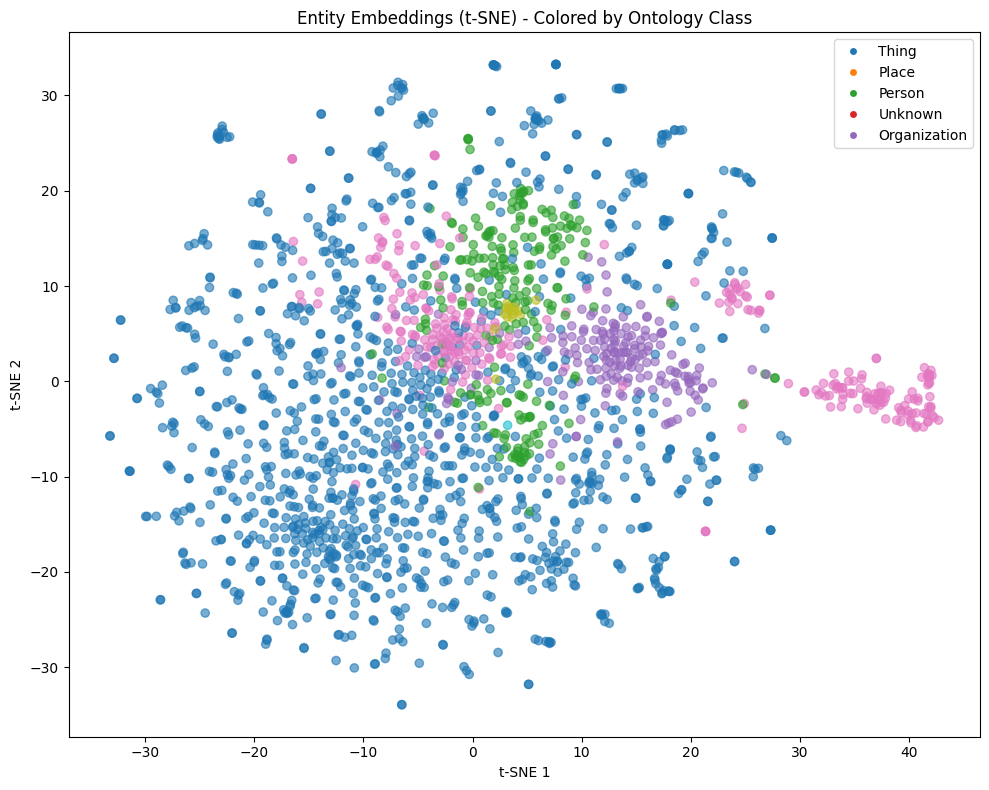
\includegraphics[width=0.95\textwidth]{../screenshots/t-SNE.png}
\caption{t-SNE visualization of entity embeddings colored by ontology class (Thing, Place, Person, Unknown, Organization).}
\label{fig:entity-embeddings-tsne}
\end{figure}

\textbf{Relation behaviour:} Symmetric relations (\texttt{dc:subject}, \texttt{dc:spatial}) challenge TransE; ComplEx handles them better. Inverse and composition relations: TransE requires $\mathbf{r}_{\mathrm{inv}}\approx-\mathbf{r}$; ComplEx uses complex space.

\subsection{Rule-Based vs.\ Embedding-Based Reasoning}
\label{sec:rule-vs-embedding}

For the SWRL rule \texttt{hasSpatialContext} (Section~3.2), we check if the embedding captures similar composition: $\mathbf{r}_{\mathrm{spatial}} + \mathbf{c}_{\mathrm{Place}}$ vs.\ relation vectors. Closest relations: \texttt{dcterms:spatial}, \texttt{wdt:P19} (place of birth). The embedding encodes partial ``spatial + Place'' structure, but rule-based reasoning remains more precise and interpretable for explicit Horn rules.

%=============================================================================
\section{RAG over RDF/SPARQL}
%=============================================================================

\subsection{Setup}

\textbf{Model:} \texttt{gemma:2b} via Ollama (REST API, \texttt{stream: false}). \textbf{Graph:} \texttt{kg\_artifacts/kb\_expanded.nt} (109,474 triples). Predicates: \texttt{dcterms:spatial}, \texttt{dc:subject}, \texttt{dc:creator}, \texttt{edm:provider}, aligned Wikidata properties.

\subsection{Schema Summary and NL$\rightarrow$SPARQL Prompt}

We build a compact schema summary: (1)~8 PREFIX declarations (\texttt{dc}, \texttt{dcterms}, \texttt{edm}, \texttt{lh}, \texttt{rdf}, \texttt{rdfs}, \texttt{owl}, \texttt{xsd}); (2)~distinct predicates (up to 80); (3)~distinct classes (up to 40); (4)~sample triples (up to 20). The prompt includes the schema, the user question, and a concrete example for location questions (e.g.\ ``Which items are linked to Romania?'' using \texttt{dcterms:spatial} and \texttt{FILTER(REGEX(...))} for multilingual place names). The LLM is instructed to return only a valid SPARQL SELECT query in a fenced \texttt{sparql} block. We extract the query with a regex and strip schema lines if present.

\textbf{Execution:} \texttt{ollama run gemma:2b} then \texttt{python src/rag/lab\_rag\_sparql\_gen.py}. File: \texttt{src/rag/lab\_rag\_sparql\_gen.py}.

\begin{lstlisting}[caption={\texttt{src/rag/lab\_rag\_sparql\_gen.py} -- schema summary and NL->SPARQL prompt}]
def build_schema_summary(g):
    preds = list_distinct_predicates(g, limit=80)
    clss = list_distinct_classes(g, limit=40)
    samples = sample_triples(g, limit=20)
SPARQL_INSTRUCTIONS = "Convert QUESTION into valid SPARQL SELECT..."
\end{lstlisting}

\subsection{Query Execution and Self-Repair}

The query is executed via rdflib; common prefixes are pre-bound. If execution fails (syntax error, unknown prefix, incomplete query), we send the error back to the LLM with the original question, bad query, and schema. The repair prompt includes an example and instructs the model to add full \texttt{SELECT ... WHERE \{ ... \}}. One repair attempt; repeated failures suggest the question is too complex.

\begin{lstlisting}[caption={Self-repair: error -> LLM -> corrected query}]
def answer_with_sparql_generation(g, schema_summary, question, try_repair=True):
    sparql = generate_sparql(question, schema_summary)
    try: vars_, rows = run_sparql(g, sparql)
    except Exception as e:
        if try_repair:
            repaired = repair_sparql(schema_summary, question, sparql, str(e))
            vars_, rows = run_sparql(g, repaired)
\end{lstlisting}

\subsection{Evaluation: Baseline vs RAG}

We evaluate five questions. For each: (1)~\textbf{LLM only}---direct answer (often hallucinated); (2)~\textbf{RAG}---SPARQL on KB, grounded results.

\begin{table}[ht]
\centering
\caption{LLM only vs.\ RAG.}
\small
\begin{tabular}{@{}p{2.4cm}p{3cm}p{3.2cm}c@{}}
\toprule
\textbf{Question} & \textbf{LLM only} & \textbf{RAG} & \textbf{OK?} \\
\midrule
Which items are linked to Romania? &
Hallucinated (Bran Castle, Danube\ldots) &
2,130 Europeana URIs via \texttt{dcterms:spatial} &
Yes \\
What places are associated with Bucharest? &
Invented places &
Items linked to \texttt{lh:Bucharest} &
Yes \\
How many items have subject archaeology? &
Approximate/false &
Exact count via \texttt{dc:subject} &
Yes \\
What entity types exist in the KB? &
Generic terms &
Person, Place, Organization, Thing, Temporal &
Yes \\
What creators appear in the base? &
Invented names &
Real creators from KB &
Yes \\
\bottomrule
\end{tabular}
\end{table}

RAG yields grounded results; the baseline hallucinates for domain-specific questions.

\begin{figure}[H]
\centering
% Portable (repo copy): compiled from \texttt{reports/} with \texttt{pdflatex report.tex}
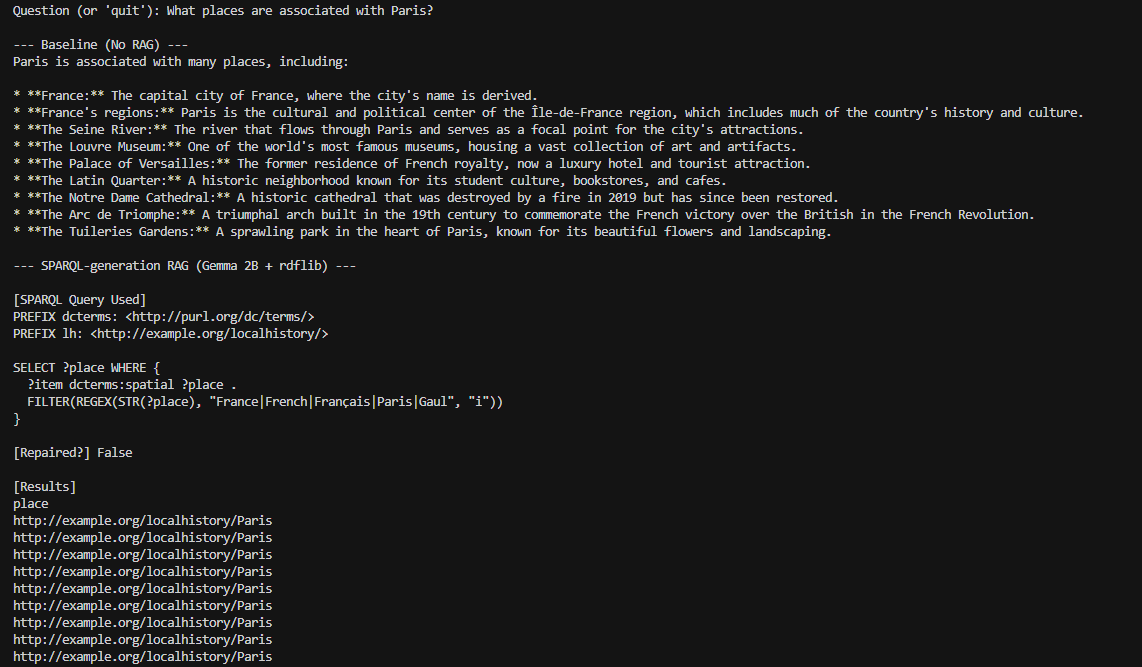
\includegraphics[width=0.95\textwidth]{../screenshots/Rag_example.png}
% Local one-off: uncomment and comment the line above if you prefer the file on Desktop
% 
\includegraphics[width=0.95\textwidth]{C:/Users/sulta/OneDrive/Bureau/Rag_example.png}
\caption{RAG demo: screenshot of baseline vs.\ SPARQL-generation output (source: \texttt{Rag\_example.png} on the project Desktop folder, copied to \texttt{screenshots/} for the PDF build).}
\end{figure}

%=============================================================================
\section{Critical Reflection}
%=============================================================================

\textbf{KB quality impact.} Predicate alignment errors introduce semantic noise. Noisy expansion from Wikidata/Europeana can add contradictory triples; cleaning (literals, URI normalization) mitigates but does not eliminate this. Ontology modelling (fine-grained vs coarse types) influences graph structure; sparse type assertions limit embedding quality.

\textbf{Noise issues.} Multilingual content (Dutch, German, Polish) causes NER errors; we use \texttt{FILTER\_ENTITIES}, \texttt{FILTER\_FRAGMENTS}, and language heuristics. Relation count is controlled by predicate whitelisting and consolidation.

\textbf{Rule-based vs embedding-based.} SWRL is deterministic and interpretable; embeddings learn from observed triples and cannot infer facts requiring external knowledge. The open-world assumption of RDF contrasts with the closed-world behaviour of embeddings.

\textbf{Improvements.} (1)~Federated SPARQL across DBpedia and Wikidata; (2)~DBpedia Spotlight for context-aware entity linking; (3)~NER/RE evaluation metrics; (4)~larger 2-hop expansion; (5)~integrating SWRL with the expanded KB in an OWL reasoner.

%=============================================================================
\section{Conclusion}
%=============================================================================

We implemented a complete pipeline from unstructured web data (Europeana API) to a structured KB aligned with Wikidata/DBpedia. Phase~1: transformer-based NER, dependency-based relation extraction. Phase~2: entity/predicate alignment, SPARQL expansion (1-hop, 2-hop, predicate-controlled), Europeana complement---109,474 triplets, 7,310 entities, 50 relations. Phase~3: OWL~DL + HermiT on \texttt{family.owl} (equivalent to the targeted SWRL rule), KGE with TransE and ComplEx (MRR 0.525 with ComplEx on the saved PyKEEN run). Phase~4: RAG with Ollama, NL$\rightarrow$SPARQL, self-repair, baseline vs RAG evaluation on five questions.

%=============================================================================
\section{Appendix: Code Mapping}
%=============================================================================

The table below allows the grader to quickly locate the code corresponding to each requirement of the grading guide.

\begin{table}[H]
\centering
\caption{Requirements $\rightarrow$ files and commands}
\resizebox{\linewidth}{!}{%
\small
\renewcommand{\arraystretch}{1.2}
\begin{tabular}{@{}lll@{}}
\toprule
\textbf{Requirement} & \textbf{File} & \textbf{Command} \\
\midrule
Crawler + ethics & \texttt{src/crawl/phase1\_crawler.py} & \texttt{python src/crawl/phase1\_crawler.py} \\
Cleaning + NER & \texttt{src/ie/phase1\_extraction.py} & \texttt{python src/ie/phase1\_extraction.py} \\
RDF + ontology & \texttt{src/kg/phase2\_build\_kb.py} & \texttt{python src/kg/phase2\_build\_kb.py} \\
Entity linking & \texttt{src/kg/phase2\_entity\_linking.py} & \texttt{python src/kg/phase2\_entity\_linking.py} \\
Predicate align. & \texttt{src/kg/phase2\_predicate\_alignment.py} & \texttt{python src/kg/phase2\_predicate\_alignment.py} \\
SPARQL expansion & \texttt{src/kg/phase2\_expand\_sparql.py}, \texttt{src/kg/phase2\_expand\_kb.py} & \texttt{python src/kg/phase2\_expand\_kb.py} \\
SWRL (family.owl) & \texttt{src/kge/phase3\_knowledge\_reasoning.ipynb} & Run the notebook \\
KGE (TransE, ComplEx) & Same & \texttt{kge\_splits/*/results.json} \\
RAG (NL$\rightarrow$SPARQL) & \texttt{src/rag/lab\_rag\_sparql\_gen.py} & \texttt{python src/rag/lab\_rag\_sparql\_gen.py} \\
\bottomrule
\end{tabular}%
}
\end{table}

%=============================================================================
\section{References}
%=============================================================================

\begin{itemize}
\item Europeana API: \url{https://pro.europeana.eu/page/search-api}
\item EDM: \url{https://pro.europeana.eu/page/edm-documentation}
\item Dublin Core: \url{https://dublincore.org/specifications/dublin-core/dcmi-terms/}
\item Wikidata: \url{https://www.wikidata.org/}, \url{https://query.wikidata.org/}
\item DBpedia: \url{https://www.dbpedia.org/}
\item PyKEEN: Ali et al., JMLR 22, 2021. \url{https://github.com/pykeen/pykeen}
\item OWLReady2: Lamy, Artificial Intelligence in Medicine 80, 2017. \url{https://owlready2.readthedocs.io/}
\item TransE: Bordes et al., NeurIPS 2013. \url{https://papers.nips.cc/paper/5071-translating-embeddings-for-modeling-multi-relational-data}
\item ComplEx: Trouillon et al., ICML 2016. \url{https://arxiv.org/abs/1606.06357}
\item Pellet: \url{https://www.w3.org/2001/sw/wiki/Pellet}
\item Ollama: \url{https://ollama.ai/}
\end{itemize}

\end{document}
